\documentclass[crop,tikz]{standalone}
\usetikzlibrary{calc}
\usetikzlibrary{arrows}
\usetikzlibrary{decorations.pathreplacing}
\begin{document}
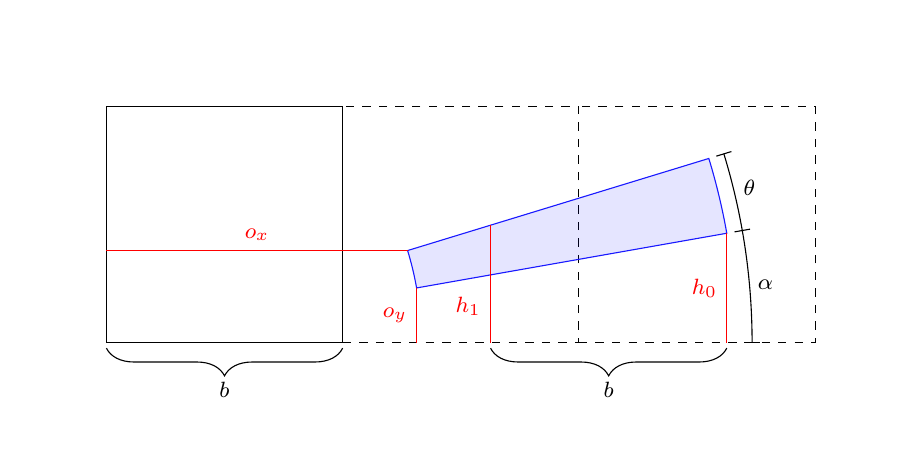
\begin{tikzpicture}
  % Constants
  \pgfmathsetmacro\b{3}
  \pgfmathsetmacro\d{8}
  \pgfmathsetmacro\c{4}
  \pgfmathsetmacro\t{7}
  \pgfmathsetmacro\a{10}
  \pgfmathsetmacro\x{\d*cos(\a)}
  \pgfmathsetmacro\y{\d*sin(\a)}
  \pgfmathsetmacro\w{\d*cos(\a)-\b}
  \pgfmathsetmacro\v{\w*tan(\a+\t)}
  \pgfmathsetmacro\ox{\c*cos(\a)}
  \pgfmathsetmacro\oy{\c*sin(\a)}
  \pgfmathsetmacro\ow{\c*cos(\a+\t)}
  \pgfmathsetmacro\ov{\c*sin(\a+\t)}
  % Boundary
  \path[use as bounding box] (0,0) rectangle (2+\b*3,2+\b);
  % Domain grids
  \draw (1,1) -- (1+\b,1) -- (1+\b,1+\b) -- (1,1+\b) -- cycle;
  \draw[dashed] (1+\b,1) -- (1+2*\b,1) -- (1+2*\b,1+\b) -- (1+\b,1+\b);
  \draw[dashed] (1+2*\b,1) -- (1+3*\b,1) -- (1+3*\b,1+\b) -- (1+2*\b,1+\b);
  % Domain size
  \draw[decorate,decoration={brace,mirror,amplitude=10pt},yshift=-2] (1,1) -- (1+\b,1) node [midway,yshift=-15] {\footnotesize $b$};
  % Lightcone
  \begin{scope}[shift={(1,1)}]
    \filldraw[fill=blue,fill opacity=0.1,draw=blue!90] (\a:\c) arc (\a:\a+\t:\c) -- (\a+\t:\d) arc (\a+\t:\a:\d) -- cycle;
    % Theta
    \draw (\a:\d+0.1) -- (\a:\d+0.3);
    \draw (\a+\t:\d+0.1) -- (\a+\t:\d+0.3);
    \draw (\a:\d+0.2) arc (\a:\a+\t:\d+0.2);
    \node at (\a+\t/2:\d+0.4) {\footnotesize $\theta$};
    % Alpha
    \draw (0:\d+0.1) -- (0:\d+0.3);
    \draw (0:\d+0.2) arc (0:\a:\d+0.2);
    \node at (\a/2:\d+0.4) {\footnotesize $\alpha$};
    % Length of c and d
    % \draw[decorate,decoration={brace,amplitude=10pt},rotate=\a+\t,yshift=20] (0,0) -- (\d,0) node [midway,xshift=-4,yshift=16] {\footnotesize $d_1$};
    % \draw[decorate,decoration={brace,amplitude=10pt},rotate=\a+\t,yshift=2] (0,0) -- (\c,0) node [midway,xshift=-4,yshift=16] {\footnotesize $d_0$};
    % Both h's
    \draw[decorate,decoration={brace,mirror,amplitude=10pt},yshift=-2] ({8*cos(10)-3},0) -- ({8*cos(10)},0) node [black,midway,yshift=-15] {\footnotesize $b$};
    \draw[red] (\x,0) -- (\x,\y) node [midway,left] {\footnotesize $h_0$};
    \draw[red] (\w,0) -- (\w,\v) node [midway,left,yshift=-8] {\footnotesize $h_1$};
    % Offsets
    \draw[red] (\ox,0) -- (\ox,\oy) node [midway,left] {\footnotesize $o_y$};
    \draw[red] (\ow,\ov) -- (0,\ov) node [midway,above] {\footnotesize $o_x$};
  \end{scope}
\end{tikzpicture}
\end{document}
